\documentclass{standalone}
\usepackage{tikz}
\usepackage{ctex,siunitx}
\setCJKmainfont{Noto Serif CJK SC}
\usepackage{tkz-euclide}
\usepackage{amsmath}
\usetikzlibrary{patterns, calc,3d}
\usetikzlibrary {decorations.pathmorphing,decorations.pathreplacing,decorations.shapes}
\begin{document}
\small
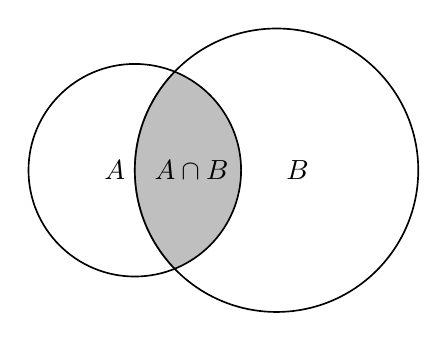
\begin{tikzpicture}[>=latex,scale=0.9]
  \tkzDefPoints{0/0/O,-1.5/0/A,0.5/0/B}
  \begin{scope}
    \tkzClipCircle(A,O)
    \tkzDrawCircle[fill=lightgray,semithick](B,A)
  \end{scope}
  \tkzInterCC(A,O)(B,A);\tkzGetPoints{C}{C'}
  \tkzDrawCircle[semithick,black](A,O)
  \tkzDrawCircle[semithick,black](B,A)
  \tkzLabelPoints[left](A)
  \tkzLabelPoints[right](B)
  \node at (-0.7,0){$A\cap B$};
\end{tikzpicture}
\end{document}